\chapter{色散与波包}\label{ch:b2:dispersion-wave-packets}

在池塘里投入一块石子，观察涟漪形成的环：新的波峰
在环的内缘产生，沿环向外传播，并在外缘消失——
整个环的移动速率慢于其中的波峰。
在远方风暴过后坐在海滩上，长而缓的涌浪
比短促的碎浪早一天到达：海洋按波长对波进行了分选。
1858 年铺设的第一条跨大西洋电报电缆，把清晰的点和
划变成了需要数分钟才能辨认的模糊信号。在这三种情形中，
波的速率都依赖于其频率：介质是
\emph{色散的}。本章引入色散关系、
同时描述传播与吸收的复波数，
一个波包（连同其能量与信息）实际传播所用的群速度，
以及电报、电视和互联网所沿用的线路——
同轴电缆。

\section{色散关系}

\begin{definition}[色散关系；相速度]\label{def:b2:dispersion-wave-packets:relation}
\index{色散关系}\index{相速度}\index{色散介质}
线性、均匀、时不变的介质允许平面
单色波 $\underline s = A\,\eu^{\iu(\omega t - kx)}$（复数记法；
物理信号取其实部），前提是 $\omega$ 与 $k$
满足该介质的\emph{色散关系} $\mathcal D(\omega, k)
= 0$，可解为 $k(\omega)$ 或 $\omega(k)$。对实数 $k$，波以
不变形地传播，其\emph{相速度}为
\[
v_\varphi = \frac\omega k .
\]
介质称为\emph{非色散的}，当 $v_\varphi$ 不依赖于
$\omega$（此时 $\omega = ck$，任何信号都无畸变地传播——
即达朗贝尔方程），否则称为\emph{色散的}。
\end{definition}

\begin{proof}
将 $\eu^{\iu(\omega t - kx)}$ 代入常系数线性方程，
$\partial_t$ 变为 $\iu\omega$，$\partial_x$ 变为
$-\iu k$，于是得到代数关系。弦、声波与
杆给出的都是 $\omega^2 = c^2k^2$。
\end{proof}

\begin{example}[色散与非色散]\label{ex:b2:dispersion-wave-packets:examples}
\index{克莱因–戈登方程}\index{深水波}
(i) 置于弹性床上的弦（单位长度受回复力 $-Ky$，
或一串单摆），$\mu\partial_t^2y = T\partial_x^2y - Ky$：$\omega^2 = \omega_c^2
+ c^2k^2$，其中 $\omega_c = \sqrt{K/\mu}$——即\emph{克莱因–戈登}
关系，与等离子体及波导中的关系相同
（\cref{ch:b2:waves-in-media,ch:b2:guided-waves}）：$v_\varphi = c/\sqrt{1 -
\omega_c^2/\omega^2} > c$，且对实数 $k$，频率低于\emph{截止频率} $\omega_c$ 时无解。
(ii) 深水重力波：$\omega^2 = gk$（在本阶段不加证明地承认），$v_\varphi =
\sqrt{g/k} = \sqrt{g\lambda/2\pi}$：长波更快——波长 \qty{100}{m} 时为
\qty{12.5}{m/s}，波长 \qty{1}{km} 时为 \qty{40}{m/s}。(iii) 原子链，$\omega =
2\omega_0|\sin(ka/2)|$（\cref{ch:b2:waves-on-strings}）。(iv) 玻璃中的光，
$k = n(\omega)\omega/c$，这就是棱镜能展开光谱的原因。
\end{example}

\begin{omfigure}
\begin{tikzpicture}
\begin{axis}[omaxis, axis x line=bottom, axis y line=left, width=6.2cm, height=4.6cm,
    xlabel={$k$}, ylabel={$\omega$}, xmin=0, xmax=3, ymin=0, ymax=3.3, xtick=\empty, ytick={1}, yticklabels={$\omega_c$}, samples=80,
    xlabel style={at={(axis description cs:1.0,0.0)}, anchor=west},
    ylabel style={at={(axis description cs:0.0,1.0)}, anchor=south},
    legend style={font=\scriptsize, at={(0.03,0.97)}, anchor=north west, draw=none, fill=none}]
  \addplot[omDef, thick, domain=0:3] {x};
  \addplot[omThm, thick, domain=0:3] {sqrt(1+x*x)};
  \addplot[omProp, thick, domain=0:3] {1.6*sqrt(x)};
  \legend{$\omega = ck$, $\omega^2 = \omega_c^2 + c^2k^2$, $\omega^2 = gk$}
\end{axis}
\end{tikzpicture}
\hfill
\begin{tikzpicture}
\begin{axis}[omaxis, axis x line=bottom, axis y line=left, width=6.2cm, height=4.6cm,
    xlabel={$\omega/\omega_c$}, ylabel={$v/c$}, xmin=0, xmax=4, ymin=0, ymax=2.6, xtick={1,2,3}, ytick={1}, samples=100,
    xlabel style={at={(axis description cs:0.5,-0.12)}, anchor=north},
    ylabel style={at={(axis description cs:-0.1,0.5)}, rotate=90, anchor=south},
    legend style={font=\scriptsize, at={(0.97,0.95)}, anchor=north east, draw=none, fill=none}]
  \addplot[omThm, thick, domain=1.08:4] {1/sqrt(1-1/(x*x))};
  \addplot[omDef, thick, domain=1.0:4] {sqrt(1-1/(x*x))};
  \addplot[black, dashed, domain=0:4] {1};
  \legend{$v_\varphi$, $v_g$}
  \node[font=\scriptsize, anchor=west, align=left] at (axis cs:0.05,1.9) {不能 \\传播};
\end{axis}
\end{tikzpicture}

{\small 左：三种色散关系——非色散介质的直线、
带截止频率的克莱因–戈登双曲线、
深水波的抛物线。右：对于克莱因–戈登关系，
相速度超过 $c$，而群速度
则小于光速，且 $v_\varphi v_g = c^2$。}
\end{omfigure}

\begin{definition}[复波数：传播与衰减]\label{def:b2:dispersion-wave-packets:complex}
\index{复波数}\index{衰减}\index{倏逝波}\index{趋肤深度}
当色散关系对实数 $\omega$ 给出复数
$\underline k = k' - \iu k''$，则波为
\[
\underline s = A\,\eu^{-k''x}\,\eu^{\iu(\omega t - k'x)} :
\]
它以 $v_\varphi = \omega/k'$ 传播，其振幅按
$\eu^{-x/\delta}$ 衰减，其\emph{衰减长度}为 $\delta = 1/k''$（它必须
沿其传播方向衰减：$k'$ 与 $k''$ 同号）。
若 $\underline k$ 为纯虚数，$\underline k = -\iu\kappa$，则波为
\emph{倏逝的}：$A\,\eu^{-\kappa x}\eu^{\iu\omega t}$，一种驻振荡，
其振幅在距离 $1/\kappa$ 内衰减殆尽，
而不传播任何东西——克莱因–戈登介质在截止频率以下的情形即属此类，
此时 $\kappa = \sqrt{\omega_c^2 - \omega^2}/c$；金属在光频下也属此类。
\end{definition}

\begin{example}[阻尼弦]\label{ex:b2:dispersion-wave-packets:damped}
置于粘性流体中的弦，$\mu\partial_t^2y + \alpha\partial_ty = T\partial_x^2y$：
$\underline k^2 = (\omega^2 - \iu\alpha\omega/\mu)/c^2$。对于弱阻尼（$\alpha \ll \mu
\omega$），$\underline k \approx \dfrac\omega c\Bigl(1 - \iu\dfrac{\alpha}{2\mu\omega}\Bigr)$：波
保持其速率，而振幅在 $\delta = 2\mu c/\alpha = 2Z/\alpha$ 的距离内衰减，
且与频率无关——这是一种\emph{耗散性的}、非色散的损耗，
每经过一个长度 $\delta$ 损失 \qty{8.7}{dB}。
\end{example}

\section{波包与群速度}

\begin{proposition}[拍；群速度]\label{prop:b2:dispersion-wave-packets:group}
\index{群速度}\index{波包}\index{拍}
两列振幅相等、频率相近的波，频率为 $\omega \pm
\delta\omega$，波数为 $k \pm \delta k$，叠加为
\[
s = 2A\cos(\delta\omega\,t - \delta k\,x)\cos(\omega t - kx) :
\]
一个以 $(\omega, k)$ 为特征的载波，以 $v_\varphi = \omega/k$ 运动，受一个缓慢的
包络调制，该包络以 $\delta\omega/\delta k$ 运动。\emph{波包}——即波数位于
$k_0$ 附近窄带内的单色波之叠加——
整体以\emph{群速度}运动，
\[
v_g = \frac{\dd\omega}{\dd k}\Bigr|_{k_0} ,
\]
此速度即其能量及所携信息的速度。
在非色散介质中 $v_g = v_\varphi = c$；否则波包在传播中会变形（即\emph{展宽}），
$\dd^2\omega/\dd k^2$ 越大，
且其频谱的补量（即空间宽度）越窄，
展宽便越快。
\end{proposition}

\begin{proof}
由和差化积公式可得拍。对于波包，记 $s =
\int a(k)\eu^{\iu(\omega(k)t - kx)}\dd k$（傅里叶叠加——傅里叶积分在
本科三年级数学分册中学习，这里仅用其作为
连续正弦和的解释），
其中 $a(k)$ 在 $k_0$ 处取峰值。将 $\omega(k) \approx \omega_0 + v_g(k - k_0)$ 展开，则
$s \approx \eu^{\iu(\omega_0t - k_0x)}\int a(k)\eu^{\iu(k - k_0)(v_gt - x)}\dd k$，
即一个载波乘以一个仅依赖于 $x - v_gt$ 的包络——
包络以 $v_g$ 运动。下一项 $\tfrac12\omega''(k_0)(k - k_0)^2t$
使各分量随时间失相，并使包络展宽。波包的能量
位于其包络所在处；任何信号亦然。
\end{proof}

\begin{omfigure}
\begin{tikzpicture}
\begin{axis}[omaxis, axis x line=middle, axis y line=none, width=13.6cm, height=4.0cm,
    xmin=0, xmax=60, ymin=-3.1, ymax=3.3, xtick=\empty, samples=600, xlabel={$x$}, clip=false,
    xlabel style={at={(axis description cs:1.0,0.5)}, anchor=west}]
  \addplot[omDef, thick, domain=0:60] {2*cos(deg(0.12*x))*cos(deg(2.2*x))};
  \addplot[omThm, thick, domain=0:60] {2*cos(deg(0.12*x))};
  \addplot[omThm, thick, domain=0:60] {-2*cos(deg(0.12*x))};
  \draw[omThm, very thick, ->] (axis cs:9,2.6) -- (axis cs:15,2.6) node[above, font=\scriptsize, pos=0.5] {$v_g$};
  \draw[omDef, very thick, ->] (axis cs:38,-2.6) -- (axis cs:48,-2.6) node[below, font=\scriptsize, pos=0.5] {$v_\varphi$};
\end{axis}
\end{tikzpicture}

{\small 拍：两个相近频率产生一个快速载波，
以相速度运动，其上叠加一个缓慢包络，以群速度运动；
在色散介质中两者速度不同，
波峰在包络中滑动。}
\end{omfigure}

\begin{example}[深水：波峰跑在群前面]\label{ex:b2:dispersion-wave-packets:deepwater}
$\omega = \sqrt{gk}$：$v_g = \tfrac12\sqrt{g/k} = \tfrac12v_\varphi$。一群涌浪
以其波峰速率的一半运动：观察一列波列时，
可以看到波峰在群的后端出现、穿过群，
并在前端消失——恰如池塘中的涟漪。一场远在 \qty{3000}{km} 之外的风暴
发出其 \qty{15}{s} 涌浪（$\lambda = gT^2/2\pi = \qty{350}{m}$，$v_g =
gT/4\pi = \qty{11.7}{m/s}$）三天后到达，其 \qty{8}{s} 波（$v_g =
\qty{6.2}{m/s}$）则在五天半后到达：海洋学家由不同
周期的到达时间来确定风暴的位置。
\end{example}

\begin{omfigure}
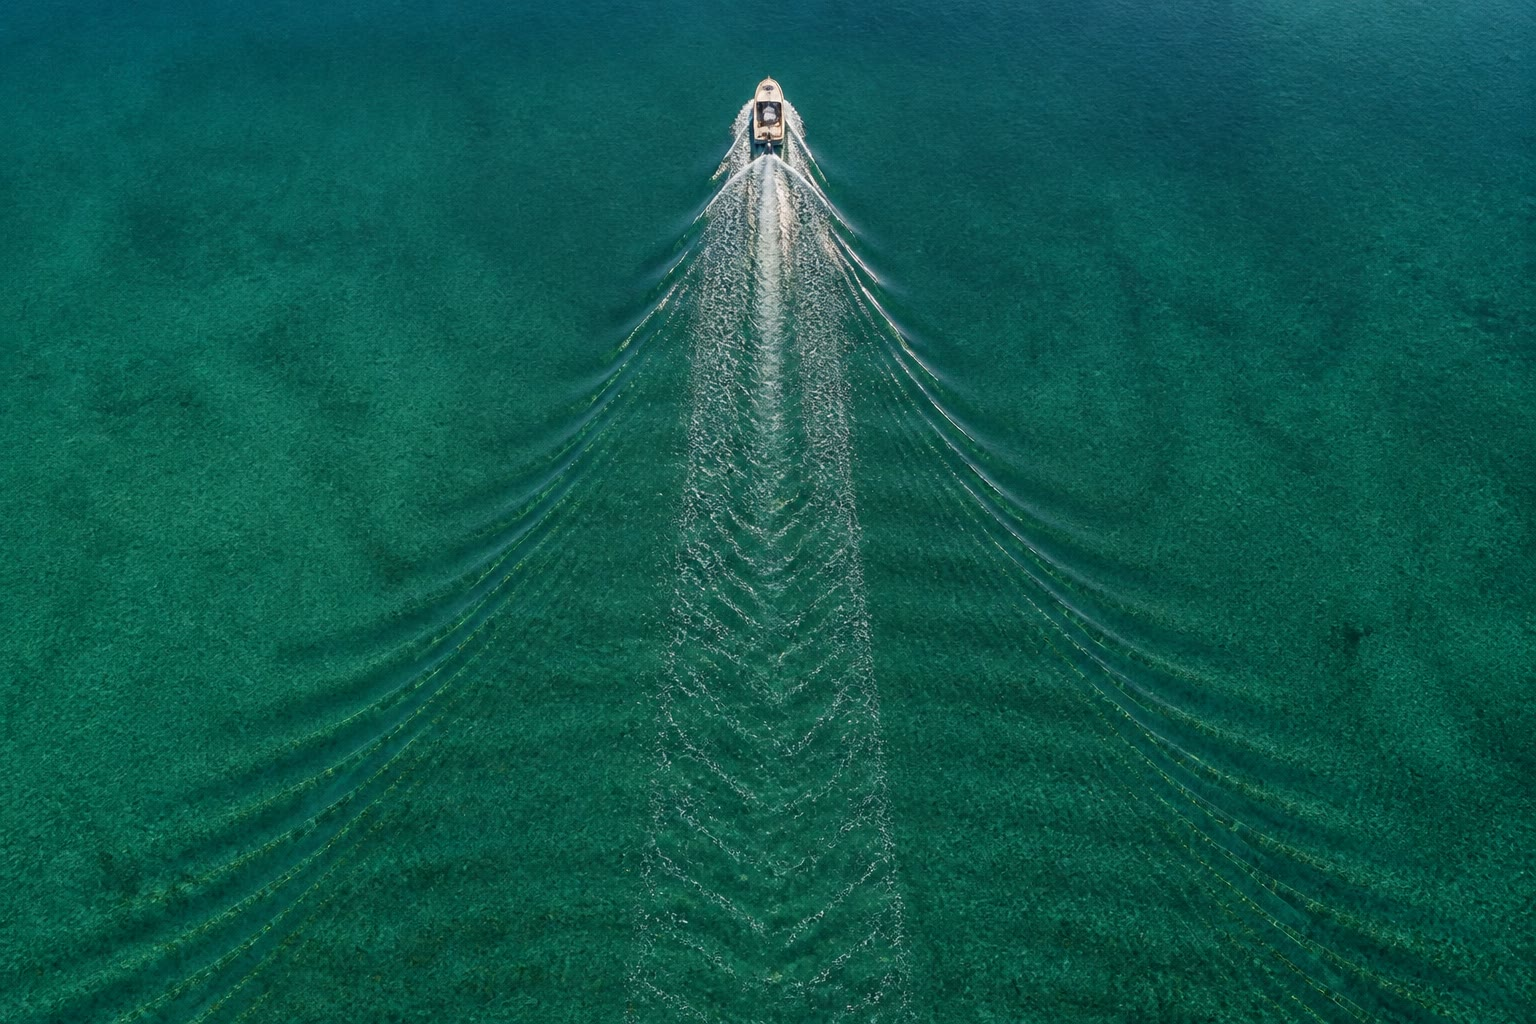
\includegraphics[width=0.56\linewidth]{images/book4/ai/b4-08-boat-wake-aerial.jpg}

{\small 平静湖面上一艘机动船的尾迹：羽毛状图样保持在固定角度的楔形区域内，因为每个水波的能量以其波峰速率的一半传播——色散的直观体现。}
\end{omfigure}


\begin{example}[克莱因–戈登：超光速，但并非如此]\label{ex:b2:dispersion-wave-packets:superluminal}
对于 $\omega^2 = \omega_c^2 + c^2k^2$：$v_\varphi = \omega/k$ 与 $v_g = c^2k/\omega$，因此
$v_\varphi v_g = c^2$：相速度超过 $c$（在电离层中，
\qty{10}{MHz} 波的波峰运动速度快于光速），但携带信号的
群速度仍低于光速。相速度既不传递能量，
也不传递信息——波峰好比灯塔光束
扫过远处云层时留下的光斑。
\end{example}

\begin{remark}[展宽]\label{rem:b2:dispersion-wave-packets:spreading}
空间宽度为 $\Delta x$ 的波包包含波数范围 $\Delta k \sim
1/\Delta x$ 内的分量（傅里叶倒易关系，在本阶段不加证明地承认）；其各分量的群速度
相差 $\Delta v_g \approx |\omega''|\Delta k$，因此经过时间 $t$ 后，它展宽了
$|\omega''|\Delta k\,t$：经过 $t_{\text{展宽}}
\sim \Delta x^2/|\omega''|$ 后宽度加倍。一个由十个 \qty{100}{m} 深水波组成的波包
（$\Delta x \approx \qty{1}{km}$，$\omega'' = -\tfrac14\sqrt{g/k^3} = \qty{-50}{m^2/s}$）
约在六小时内宽度加倍；一个 \qty{1}{ns} 的光脉冲在光纤中
每公里展宽数十皮秒——这是
长距离链路比特率的极限。
在\cref{ch:b2:schrodinger-wave-functions}中的量子波包也因同样的原因展宽。
\end{remark}

\section{同轴电缆}

\begin{proposition}[电报方程；无损线]\label{prop:b2:dispersion-wave-packets:coax}
\index{同轴电缆}\index{电报方程}\index{特征阻抗}\index{传输线}
同轴电缆（或任一双导体线）单位长度上具有
电感 $\Lambda$ 和电容 $\Gamma$。两导体之间的电压 $v(x, t)$
与内导体中的电流 $i(x, t)$ 满足
\emph{电报方程}
\[
\frac{\partial v}{\partial x} = -\Lambda\frac{\partial i}{\partial t} , \qquad
\frac{\partial i}{\partial x} = -\Gamma\frac{\partial v}{\partial t} ,
\]
由此可得 $v$ 与 $i$ 满足达朗贝尔方程，其中
\[
c = \frac1{\sqrt{\Lambda\Gamma}} , \qquad
v = Z_c\,i \ \text{波传向 } +x, \quad Z_c = \sqrt{\frac\Lambda\Gamma} ,
\]
$Z_c$ 称为线路的\emph{特征阻抗}。对于
半径为 $a < b$ 的同轴电缆，填充有相对介电常数为
$\varepsilon_r$ 的电介质，$\Lambda = \dfrac{\mu_0}{2\pi}\ln\dfrac ba$，$\Gamma =
\dfrac{2\pi\varepsilon_0\varepsilon_r}{\ln(b/a)}$，故 $c = c_0/\sqrt{\varepsilon_r}$（约为
\qty{2e8}{m/s}，即光速的三分之二），且 $Z_c = \dfrac{60\,\Omega}
{\sqrt{\varepsilon_r}}\ln\dfrac ba$：常用电缆为 \qty{50}{\ohm} 或 \qty{75}{\ohm}。
\end{proposition}

\begin{proof}
将小段 $[x, x + \dd x]$ 建模为串联电感 $\Lambda\dd x$ 与
并联电容 $\Gamma\dd x$：该段上的电压降为
$\Lambda\dd x\,\partial_ti$，流入电容的电流为 $\Gamma\dd x
\,\partial_tv$。交叉求导。对 $v = f(x - ct)$，第一式
给出 $i = f(x - ct)/\Lambda c = v/\sqrt{\Lambda/\Gamma}$。$\Lambda$ 与
$\Gamma$ 的值与本科一年级分册中算出的圆柱形电容器及同轴线
电感的结果相同。
\end{proof}

\begin{omfigure}
\begin{tikzpicture}[font=\small]
  \begin{scope}
    \draw (0,0) to[L, l=$\Lambda\,\dd x$] (2.2,0) to[C, l=$\Gamma\,\dd x$] (2.2,-1.6);
    \draw (0,-1.6) -- (2.2,-1.6);
    \draw (2.2,0) -- (3.8,0); \draw (2.2,-1.6) -- (3.8,-1.6);
    \draw[->] (0.1,0.35) -- (0.7,0.35); \node[font=\footnotesize] at (0.4,0.6) {$i(x)$};
    \draw[->] (2.9,0.35) -- (3.5,0.35); \node[font=\footnotesize] at (3.2,0.6) {$i(x+\dd x)$};
    \node[font=\footnotesize] at (-0.3,-0.8) {$v(x)$}; \node[font=\footnotesize] at (4.6,-0.8) {$v(x+\dd x)$};
    \draw (-0.6,-0.2) -- (-0.6,-1.4); \draw[->] (-0.6,-1.4) -- (-0.6,-0.3);
    \node[font=\footnotesize] at (1.6,-2.3) {线路的一小段};
  \end{scope}
  \begin{scope}[xshift=8.4cm, yshift=-0.8cm]
    \draw[thick, fill=omExo!30] (0,0) circle (1.3);
    \draw[thick, fill=omDef!15] (0,0) circle (1.05);
    \draw[thick, fill=omThm!40] (0,0) circle (0.3);
    \draw[<->] (0,0) -- (30:0.3) node[pos=1.6, font=\footnotesize] {$a$};
    \draw[<->] (0,0) -- (-50:1.05) node[pos=0.6, right, font=\footnotesize] {$b$};
    \node[font=\footnotesize] at (0,1.65) {$\varepsilon_r$ 介质、编织层、内芯};
    \node[font=\footnotesize] at (0,-1.75) {$Z_c = \dfrac{60\,\Omega}{\sqrt{\varepsilon_r}}\ln\dfrac ba$};
  \end{scope}
\end{tikzpicture}

{\small 左：无损线路一小段 $\dd x$ 的等效电路——串联电感、并联
电容——由此导出电报方程。右：同轴电缆的截面图，其
$\Lambda$ 与 $\Gamma$ 仅
取决于半径之比，
以及介质。}
\end{omfigure}

\begin{omfigure}
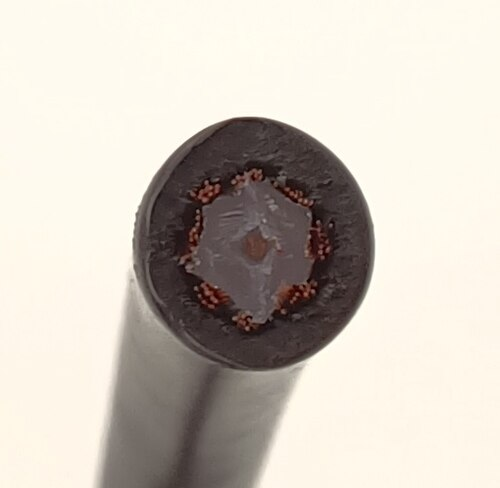
\includegraphics[width=0.46\linewidth]{images/book3/coaxial-cable.jpg}

{\small 同轴电缆：内芯、介质、编织外导体——一种传输线，其每米的电感与电容决定了它的速度与特性阻抗。}
\end{omfigure}

\begin{proposition}[有耗线；无畸变条件]\label{prop:b2:dispersion-wave-packets:lossy}
\index{赫维赛德条件}\index{开尔文平方律}
若单位长度上串联电阻为 $R$，
并联电导为 $G$，则方程变为 $\partial_xv = -\Lambda\partial_ti - Ri$，$\partial_xi =
-\Gamma\partial_tv - Gv$，色散关系为 $\underline k^2 = (\Lambda\omega -
\iu R)(\Gamma\omega - \iu G)$：该线路有色散且有衰减。两种极限如下：
(i) 若 $R/\Lambda = G/\Gamma$（赫维赛德条件，可通过增加电感达到），
则 $\underline k = \omega\sqrt{\Lambda\Gamma} - \iu\sqrt{RG}$，各频率以相同速度、
相同衰减传播——线路\emph{衰减}但不\emph{畸变}。(ii) $\Lambda \approx 0$，$G \approx 0$
（最早的海底电缆）：$\partial_x^2v = R\Gamma\,\partial_tv$，
即\emph{扩散}方程——脉冲并不传播，而是逐渐展宽，
到达距离 $L$ 处所需时间约为 $\sim R\Gamma L^2$，
（开尔文平方律），
电缆长十倍，所需时间则长一百倍。
\end{proposition}

\begin{proof}
代入 $\eu^{\iu(\omega t - kx)}$：$-\iu kv = -(\iu\omega\Lambda + R)i$，$-\iu ki = -(\iu
\omega\Gamma + G)v$；两式相乘。在赫维赛德条件下，乘积为一个
完全平方。扩散极限下略去 $\iu\omega\Lambda$ 与 $G$ 项。
\end{proof}

\begin{example}[三条电缆]\label{ex:b2:dispersion-wave-packets:cables}
1858 年的跨大西洋电缆：单根铜线包裹在古塔胶中，
$R \approx \qty{3}{\ohm/km}$, $\Gamma \approx \qty{0.3}{\micro F/km}$, $L = \qty{3000}{km}$:
$R\Gamma = \qty{9e-10}{s/m^2}$，$R\Gamma L^2 \approx \qty{8}{s}$（每点），每分钟仅
能发一个字。操作员试图以 \qty{2}{kV} 强行驱动信号，结果
数周内便击穿了绝缘层。一条电话线
每隔 \qty{2}{km} 加装线圈，以满足赫维赛德条件
（1900 年）：可清晰通话的距离达数百千米。现代的 \qty{50}{\ohm}
同轴电缆：$c = \qty{2e8}{m/s}$，$\Lambda = \qty{0.25}{\micro H/m}$，$\Gamma =
\qty{100}{pF/m}$，衰减由导体中的
趋肤效应引起（见\cref{ch:b2:waves-in-media}），随 $\sqrt f$ 增大：
在 \qty{100}{MHz} 下每百米仅几分贝。
\end{example}

\begin{method}[读懂色散关系]\label{met:b2:dispersion-wave-packets:method}
(1) 用复数记号写出介质的波动方程，
并解出 $\underline k(\omega)$。(2) 若 $k$ 为实数，计算 $v_\varphi = \omega/k$ 与
$v_g = \dd\omega/\dd k$（或 $1/(\dd k/\dd\omega)$），比较：是否色散，
为正常色散（$v_g < v_\varphi$）还是反常色散。(3) 若 $k$ 为复数，分为
传播部分（$k'$）与衰减部分（$k''$，长度为 $1/k''$）；若
为纯虚数，则为倏逝波，无输运。(4) 截止频率
将传播频带与倏逝频带分开。(5) 对信号而言，
应依据速度 $v_g$ 下的包络分析，切不可依据波峰推断。
\end{method}

\section{练习}

\begin{exercise}[$\star$]\label{exo:b2:dispersion-wave-packets:1}
深水波，$\omega^2 = gk$。(a) 求 \qty{100}{m} 涌浪的相速度、群速度与
周期。(b) 对周期为 \qty{14}{s} 的涌浪，求
其波长、$v_\varphi$、$v_g$，以及其能量穿越 \qty{5000}{km} 所需的时间。
(c) 为什么周期为 \qty{2}{s} 的小浪根本到不了那里？
\end{exercise}

\begin{exercise}[$\star$]\label{exo:b2:dispersion-wave-packets:2}
某介质满足 $\omega^2 = \omega_c^2 + c^2k^2$，其中 $\omega_c = 2\pi \times \qty{1e7}{rad/s}$
$c = \qty{3e8}{m/s}$。当 $f = \qty{20}{MHz}$ 时，求 $k$、$v_\varphi$、$v_g$ 以及
它们的乘积。当 $f = \qty{5}{MHz}$ 时，求 $\kappa$ 与穿透深度。
\end{exercise}

\begin{exercise}[$\star$]\label{exo:b2:dispersion-wave-packets:3}
两个音叉的频率分别为 \qty{440}{Hz} 与 \qty{444}{Hz}：求拍频，以及
响度变化的周期。两列水波的波长分别为
\qty{100}{m} 与 \qty{110}{m}：求其频率、波长以及
包络的速度；并与 \qty{105}{m} 处的 $v_g$ 作比较。
\end{exercise}

\begin{exercise}[$\star$]\label{exo:b2:dispersion-wave-packets:4}
同轴电缆：内导体直径 \qty{0.9}{mm}，外导体直径
\qty{3.0}{mm}，填充聚乙烯（$\varepsilon_r = 2.3$）。求 $\Lambda$、$\Gamma$、波速、
特性阻抗、每米延迟，以及与 \qty{10}{ns} 延迟等效的电缆长度；
并求同一电缆改用空气时的结果。
\end{exercise}

\begin{exercise}[$\star\star$]\label{exo:b2:dispersion-wave-packets:5}
\emph{刚性弦。} 实际钢琴弦满足 $\mu\partial_t^2y = T\partial_x^2y
- EI\,\partial_x^4y$（$EI$ 为弯曲刚度）。(a) 求色散关系、
相速度与群速度。(b) 对 A$_4$ 弦（见\cref{ch:b2:waves-on-strings}，
其参数为 $T = \qty{685}{N}$，$\mu = \qty{6.1}{g/m}$，$EI =
\qty{9.8e-3}{N.m^2}$），求第八阶谐音的 $v_\varphi$ 相对增量；
其中 $k = 8\pi/L$，$L = \qty{0.38}{m}$；并与该章求得的
非谐性进行核对。(c) 色散是正常的还是反常的？尖锐的拨弦
经过若干次往返后会呈现什么样子？
\end{exercise}

\begin{exercise}[$\star\star$]\label{exo:b2:dispersion-wave-packets:6}
\emph{阻尼弦。} $\mu\partial_t^2y + \alpha\partial_ty = T\partial_x^2y$。(a) 推导
色散关系。(b) 当 $\alpha \ll \mu\omega$ 时，证明 $k' \approx \omega/c$，并且
$k'' \approx \alpha/2Z$；求以分贝每米表示的衰减。(c) 数值：$\mu =
\qty{5}{g/m}$，$T = \qty{50}{N}$，$\alpha = \qty{0.02}{kg.m^{-1}.s^{-1}}$，$f =
\qty{100}{Hz}$：检验近似是否成立，并求 $\delta$。(d) 阻尼
弦是否为色散的？$\alpha$ 处于何种范围时它会变为色散的？
\end{exercise}

\begin{exercise}[$\star\star$]\label{exo:b2:dispersion-wave-packets:7}
\emph{涟漪。} 短水波由表面张力主导：$\omega^2 =
\gamma k^3/\rho$（$\gamma = \qty{0.072}{N/m}$）；完整关系为 $\omega^2 = gk +
\gamma k^3/\rho$。(a) 求纯毛细波的 $v_\varphi$ 与 $v_g$，
哪一个更大？(b) 证明完整关系的相速度
在 $\lambda_m = 2\pi\sqrt{\gamma/\rho g}$ 处取极小值，并计算 $\lambda_m$ 与 $v_{\min}$。
(c) 船速低于 $v_{\min}$ 时不产生尾波，原因何在？(d) 雨滴落在
池塘上形成环状波纹，其波峰落后于环：这是何种情形？
\end{exercise}

\begin{exercise}[$\star\star$]\label{exo:b2:dispersion-wave-packets:8}
\emph{展宽。} 初始宽度为 $\Delta x_0$ 的波包，其宽度将
经过 $t_{\text{展宽}} \approx \Delta x_0^2/|\omega''(k_0)|$ 后加倍。(a) 一组深水
波，波长 $\lambda = \qty{50}{m}$，$\Delta x_0 = \qty{500}{m}$。(b) 一个光脉冲在
玻璃光纤中：$\omega'' \approx \qty{-0.16}{m^2/s}$；一个 \qty{10}{ps} 脉冲（$\Delta x_0 =
\qty{2}{mm}$）：展宽所需时间，以及此期间行进的距离；对同样的
\qty{1}{ns} 脉冲，同样求解。为何长距离光链路要用更长的脉冲或
色散补偿光纤？
\end{exercise}

\begin{exercise}[$\star\star$]\label{exo:b2:dispersion-wave-packets:9}
\emph{海底电缆。} $R = \qty{3}{\ohm/km}$，$\Gamma = \qty{0.3}{\micro F/km}$，
$\Lambda$ 与 $G$ 可忽略。(a) 证明 $v$ 满足扩散方程，并
求其扩散系数。(b) 求色散关系 $\underline k(\omega)$；求相速度
与衰减长度，分别在 \qty{1}{Hz} 与 \qty{10}{Hz} 处的值。(c)
求信号在 \qty{3000}{km} 上“到达”所需的时间（$\sim R\Gamma L^2$），并求
以每分钟字数计的速率。(d) 赫维赛德的补救办法：
要使 $R/\Lambda = G/\Gamma$ 成立（若 $G = \qty{1e-7}{S/km}$），每千米所需的电感为多少？为何当初难以加入？
\end{exercise}

\begin{exercise}[$\star\star\star$]\label{exo:b2:dispersion-wave-packets:10}
\emph{能量以群速度传播。} 弹性床上的弦：
$\mu\partial_t^2y = T\partial_x^2y - Ky$，波 $y = A\cos(\omega t - kx)$，且 $\omega^2 =
\omega_c^2 + c^2k^2$。(a) 求能量密度 $e = \tfrac12\mu(\partial_ty)^2 + \tfrac12T
(\partial_xy)^2 + \tfrac12Ky^2$ 与通量 $\mathcal P = -T\partial_xy\,\partial_ty$：验证
$\partial_te + \partial_x\mathcal P = 0$。(b) 求该波的时间平均 $\langle e\rangle$ 与
$\langle\mathcal P\rangle$。(c) 证明 $\langle\mathcal P\rangle/
\langle e\rangle = c^2k/\omega = v_g$，而非 $v_\varphi$。(d) 截止频率以下的
能量通量会发生什么变化？
\end{exercise}

\begin{exercise}[$\star\star\star$]\label{exo:b2:dispersion-wave-packets:11}
\emph{涌浪与海啸。} 波长为 $\lambda$ 的水波位于深度 $h$ 处，
满足 $\omega^2 = gk\tanh kh$（在本阶段不加证明地承认）。(a) 求深水与
浅水（$kh \ll 1$）极限下的结果；浅水波的速率；它们是否
为色散的？(b) 一次波长 $\lambda = \qty{200}{km}$ 的海啸，位于水深 \qty{4}{km} 的海洋中：
属于哪一极限，求其速率与周期；穿越 \qty{8000}{km} 所需的时间。(c) 其
离岸振幅为 \qty{0.5}{m}：求单位波峰长度的能量
（承认单位面积能量 $E = \tfrac12\rho gA^2$），对 \qty{1000}{km} 的波前，
当水深降至 \qty{10}{m} 时会发生什么，若能量通量 $Ev_g$ 守恒
（格林定律，$A \propto h^{-1/4}$）？(d) 波长为 \qty{100}{m} 的涌浪
抵达海滩，在何种水深处开始感受到海底的影响，
以及其波峰为何会转为与海岸平行？
\end{exercise}

\begin{exercise}[$\star\star\star$]\label{exo:b2:dispersion-wave-packets:12}
\emph{线上的脉冲。} 一根 \qty{50}{\ohm} 的电缆，长 $\ell = \qty{100}{m}$，
（$c = \qty{2e8}{m/s}$），在 $x = 0$ 端由内阻为
\qty{50}{\ohm} 的信号源供电，并在 $x = \ell$ 端接负载 $R_L$。(a) 证明
到达末端的波被反射，其电压反射系数
为 $r = (R_L - Z_c)/(R_L + Z_c)$（将 $v$ 与 $i$ 写成入射波
与反射波之和，并在负载上应用欧姆定律）。(b) 求下列取值的结果：
$R_L = 50$、$0$、$\infty$、\qty{150}{\ohm}。(c) 发出一个 \qty{1}{ns}、\qty{1}{V} 的脉冲，
求各负载情形下信号源端示波器所显示的内容及出现时刻；
并说明信号源的 \qty{50}{\ohm} 内阻为何重要。(d) 埋地电缆中的一处故障
经 \qty{1.8}{\micro s} 后回波返回，故障位于何处？（时域
反射法。）
\end{exercise}

\section{问题：电缆与大海}

\begin{problem}[{周末问题——色散的作用：使点信号模糊的电报电缆，
预示风暴的涌浪，横越大洋的海啸，
以及不断展宽的波包}]
\label{pb:b2:dispersion-wave-packets:1}

\medskip
\noindent\textbf{第一部分——电报电缆。}
1866 年跨大西洋电缆：$R = \qty{2.0}{\ohm/km}$，$\Gamma = \qty{0.25}{\micro F/km}$，
$\Lambda = \qty{0.5}{mH/km}$，$G$ 可忽略，长度 $L = \qty{3500}{km}$。
\begin{enumerate}
  \item 写出含 $R$ 的电报方程，并导出
        色散关系 $\underline k^2 = \Gamma\omega(\Lambda\omega - \iu R)$。
  \item 在何频率下 $\Lambda\omega$ 等于 $R$？由此可得：
        对电报频率（几赫兹）而言，线路处于
        扩散区。
  \item 在该区域中，$\underline k = \sqrt{-\iu R\Gamma\omega}$：求 $k'$ 与 $k''$
        （注意 $\sqrt{-\iu} = (1 - \iu)/\sqrt2$）；求相速度与
        衰减长度，分别在 \qty{1}{Hz} 与 \qty{4}{Hz} 处的值。
  \item 求整条电缆以分贝计的衰减，分别在 \qty{1}{Hz} 与
        \qty{4}{Hz} 处的值。哪一频率得以保留？这对尖锐的
        点信号有何影响？
  \item 开尔文对渡越时间的估计，$R\Gamma L^2$；并求实际
        速率（以每分钟字数计）；若一个字约含
        $10$ 个点和划，且点不得重叠。
  \item 赫维赛德建议增大 $\Lambda$：取何值可使 $\Lambda\omega = R$
        在 \qty{4}{Hz} 时成立，此时速率与衰减分别为多少
        （取 $G = 0$，故条件 $R/\Lambda = G/\Gamma$ 无法
        精确满足，需在该频率下使用一般关系式）？
  \item 现代光纤的传输速率为 \qty{1e10}{bit/s}：
        与第 5 小题相比较，以 10 的幂次表示。
\end{enumerate}

\medskip
\noindent\textbf{第二部分——涌浪。}
深水情形：$\omega^2 = gk$。
\begin{enumerate}[resume]
  \item 相速度与群速度作为周期 $T$ 的函数。
  \item 一场风暴距海岸 \qty{4000}{km}，产生周期从
        \qty{6}{s} 到 \qty{18}{s} 的波：求每个极值的到达时间；
        以及涌浪事件的持续时间。
  \item 证明：在距风暴 $D$ 的海岸，到达的周期满足
        $1/T = gt/4\pi D$，其中 $t$ 从风暴发生时刻起算：$1/T$
        随时间线性增长。某浮标在某日正午记录 $T = \qty{16}{s}$，
        而恰好 \qty{24}{h} 后记录 $T = \qty{12}{s}$，
        求风暴的距离。
  \item 振幅为 $A$ 的涌浪，单位面积能量为 $\tfrac12\rho
        gA^2$；穿过 \qty{1}{m} 波峰线的功率，取 $A =
        \qty{1.5}{m}$、$T = \qty{12}{s}$。（用群速度——为什么？）
  \item 一座波浪能电站，波前长 \qty{1}{km}，效率 $30\%$：
        求电功率；与风力涡轮机（\qty{3}{MW}）相比较。
  \item 一条船在深水中以 \qty{5}{m/s} 速度航行，身后留下
        静止的尾迹：哪一波长的相速度等于船速，因而随船运动？
        为什么图样呈
        V 形拖尾，且比波峰自身展开所暗示的更窄
        （考虑 $v_g = v_\varphi/2$）？
  \item 站在悬崖上观察一组涌浪，描述单个波峰
        在该组波经过固定浮标期间的运动；
        时长为 \qty{2}{min} 的一组波包含多少个波峰，
        （$T = \qty{12}{s}$），这些波峰相当于
        多少个波峰的“寿命”？
\end{enumerate}

\medskip
\noindent\textbf{第三部分——海啸。}
$\omega^2 = gk\tanh kh$；太平洋深度 $h = \qty{4.0}{km}$。
\begin{enumerate}[resume]
  \item 一次地震使一块 \qty{100}{km} 宽的海床
        抬升 \qty{2}{m}；波长 $\lambda \approx \qty{200}{km}$，
        验证其为浅水波，并求其速率、周期，以及
        到达 \qty{6000}{km} 外海岸所需的时间。
  \item 它是色散波吗？与第二部分的涌浪相比：
        它比涌浪更早还是更晚到达？哪一种以
        单一脉冲的形式到达？
  \item 离岸处其高度为 \qty{0.6}{m}：求单位面积的能量；
        长 \qty{500}{km} 的波前、在一个波长内展开的总能量；
        并与 \qty{1}{Mt} 的爆炸（\qty{4.2e15}{J}）比较。
  \item 格林定律：水深降至近岸 \qty{20}{m} 时的波高
        （能流 $\tfrac12\rho gA^2v_g$ 守恒，$v_g = \sqrt{gh}$）；
        该处的速率与波长；为什么波随后变陡，
        并像墙一样破碎。
  \item 一艘在海上的船为何察觉不到海啸经过？
  \item 相距 \qty{6000}{km} 的验潮仪记录了该波：
        走时给出了什么？为什么在深度变化的海洋上，
        测得的速率略小于 $\sqrt{gh}$？
\end{enumerate}

\medskip
\noindent\textbf{第四部分——扩散的波包。}
\begin{enumerate}[resume]
  \item 对深水，计算 $\omega''(k) = \dd^2\omega/\dd k^2$，
        并求 $\lambda = \qty{100}{m}$ 时的值。
  \item 释放一个由 \qty{10}{} 个此类波组成的波包（$\Delta x_0 \approx \qty{1}{km}$），
        扩散时间为 $\Delta x_0^2/|\omega''|$；
        这段时间内该波包所走的距离。
  \item 用文字解释：谱宽较窄（即波列较长）的波包
        为何扩散较慢，以及第三部分的海啸
        为何几乎不扩散。
  \item 对波长为 \qty{0.1}{nm} 的电子作同样估计，
        其局域在 \qty{1}{nm} 范围内，$\omega = \hbar k^2/2m$（$\hbar =
        \qty{1.05e-34}{J.s}$，$m = \qty{9.1e-31}{kg}$）：求扩散时间与
        所走距离——这是首次与量子
        \cref{ch:b2:schrodinger-wave-functions}中的波包相接触。
  \item 用表格总结：对于电缆、涌浪、海啸和电子，
        色散关系、$v_\varphi$、$v_g$，以及
        介质是扩散还是仅衰减。
\end{enumerate}
\end{problem}
